\chapter{Applicazioni lineari}
\section{Definizione}
\begin{definizione} \label{d:applicazione-lineare}
	Siano $V$ e $Z$ due spazi vettoriali su un campo $K$.
	Si definisce \emph{applicazione lineare} una funzione $T\colon V\to Z$ omogenea e additiva, ossia per la quale $\forall  x,  y\in V$ e $\lambda\in K$, si ha
	\begin{equation*}
		T(x+y)=T(x)+T(y)\qeq T(\lambda x)=\lambda T(x),
	\end{equation*}
	dove i primi membri delle uguaglianze sono operazioni in $V$, e i secondi sono operazioni in $Z$ (indicando con $+$ e $\cdot$ le due operazioni interne per entrambi gli spazi).
\end{definizione}
Le applicazioni lineari sono dunque degli omomorfismi tra spazi vettoriali, in quanto ne preservano la struttura data dalle operazioni interne.
Per linearità, vale sempre la relazione $T(0_V)=0_Z$, poiché $T(0_V)=T(0_V+0_V)=T(0_V)+T(0_V)$, da cui $T(0_V)=0_Z$ sottraendo $T(0_V)$ a entrambi i membri: quest aè una condizione facile da usare per verificare la linearità di una data funzione.
L'insieme delle applicazioni lineari da $V$ a $Z$ (entrambi basati sullo stesso campo) è indicato con $\lin(V,Z)$.
In esso possiamo definire l'addizione e la moltiplicazione per uno scalare come
\begin{equation*}
	(T+S)(v)\defeq T(v)+S(v),\hspace{2cm}(\lambda T)(v)\defeq \lambda \big(T(v)\big)
\end{equation*}
per $T,S\in\lin(V,Z)$, $v\in V$ e $\lambda\in K$.
Dotato di queste operazioni, $\lin(V,Z)$ è uno spazio vettoriale sul campo $K$.
L'elemento neutro dell'addizione è l'applicazione (evidentemente lineare) che manda ogni elemento di $V$ in $0_Z$, anche detta \emph{applicazione nulla}.

\paragraph{Esempi}
\begin{itemize}
	\item L'applicazione identità di $V$, indicata spesso con $I_V$, per la quale $I_V(v)=v$ per ogni $v\in V$, è ovviamente lineare.
	\item Sia $W$ un sottospazio di $V$: chiamiamo \emph{proiezione canonica} in $W$ la funzione $\pi\colon V\to V\quot W$ che ad ogni $v\in V$ associa la classe di equivalenza $[v]_W=W+v$.
		Tale funzione è additiva in quanto per $a,b\in V$, $\pi(a+b)=W+(a+b)=(W+a)+(W+b)=\pi(a)+\pi(b)$.
		È anche omogenea perch\'e $\pi(\lambda a)=W+\lambda a=\lambda(W+a)=\lambda\pi(a)$.
		La funzione $\pi$ è quindi un'applicazione lineare.
	\item La funzione $f\colon\R^2\to\R^2$ data da $f([x,y]^T)=[x+y,y+1]^T$ non è un'applicazione lineare, poich\'e $f([0,0]^T)=[0,1]^T\ne[0,0]^T$.
\end{itemize}

Un'applicazione lineare da uno spazio in s\'e stesso è detta \emph{endomorfismo} (lineare), e indichiamo l'insieme degli endomorfismi di uno spazio $V$ con $\End(V)$.
In questo insieme possiamo definire un'ulteriore operazione, la composizione tra endomorfismi: con essa $\End(V)$ assume l'ulteriore struttura di \emph{algebra}, sempre sul campo $K$.
L'elemento neutro di $\End(V)$ è l'identità $I_V$, come nell'esempio precedente, che associa ogni elemento di $V$ a s\'e stesso, ed è tale che $I_V\circ T=T\circ I_V=T$ per ogni $T\in\End(V)$.

L'iniettività e la suriettività delle applicazioni lineari sono definite allo stesso modo di una qualsiasi funzione.
In particolare, un'applicazione lineare che è sia iniettiva che suriettiva è detta \emph{isomorfismo lineare} (o solo isomorfismo).
Due spazi vettoriali $V$ e $Z$ legati da un isomorfismo $T\colon V\to Z$ sono detti \emph{isomorfi}, e si indica ciò con la scrittura $V\cong Z$.

Come ogni omomorfismo, definiamo un nucleo anche per le applicazioni lineari.
\begin{definizione} \label{d:nucleo-applicazione-lineare}
	Si definisce \emph{nucleo} dell'omomorfismo $T$ l'insieme degli elementi $x\in V$ tali per cui $T(x)=0_Z$:
	\begin{equation*}
		\Ker T=\{x\in V\colon T(x)=0_Z\}.
	\end{equation*}
\end{definizione}
La linearità permette una facile verifica dell'iniettività di un'applicazione lineare.
\begin{teorema} \label{t:iniettivita-nucleo}
	Un'applicazione lineare $T\in\lin(V,Z)$ è iniettiva se e solo se $\Ker T=\{0_V\}$.
\end{teorema}
\begin{proof}
	Per ogni applicazione lineare vale $T(0_V)=0_Z$, come già visto.
	Per l'iniettività, ogni $z\in Z$ ha un'unica controimmagine, quindi l'unico $v\in V$ per cui $T(v)=0_Z$ è proprio $0_V$, di conseguenza $\Ker T=\{0_V\}$.

	Viceversa, ipotizziamo $\Ker T=\{0_V\}$.
	Se $T(v)=T(w)$ allora $T(v)-T(w)=0_Z$, e per linearità si ha $T(v-w)=0_Z$, cioè $v-w\in\Ker T$.
	Ma $\Ker T=\{0_V\}$ implica $v-w=0_V$, dunque $v=w$ e $T$ è iniettiva.
\end{proof}

\begin{definizione} \label{d:immagine-applicazione-lineare}
	Sia $T\in\lin(V,Z)$.
	Si definisce \emph{immagine} di $T$ l'insieme degli elementi $z\in Z$ per i quali esiste una controimmagine $v\in V$:
	\begin{equation*}
		\Imm T=\{z\in Z\colon\exists v\in V\colon T(v)=z\}.
	\end{equation*}
\end{definizione}
Sia il nucleo che l'immagine di un omomorfismo $T\in\lin(V,Z)$ sono sottospazi vettoriali, rispettivamente di $V$ e di $Z$.
Infatti:
\begin{itemize}
	\item Siano $v,w\in\Ker T$ e $\lambda \in K$.
		Allora $T(v+w)=T(v)+T(w)=0_Z+0_Z=0_Z$, e $T(\lambda v)=\lambda T(v)=\lambda 0_Z=0_Z$, quindi $v+w,\lambda v\in\Ker T$.
	\item Siano $y,z\in\Imm T$ e $\mu\in K$.
		Esistono due vettori $a,b\in V$ per i quali $T(a)=y$ e $T(b)=z$.
		Allora $z+y=T(a)+T(b)=T(a+b)$, cioè $z+y$ è l'immagine di un elemento $a+b$, che appartiene ancora a $V$; analogamente $T(\mu a)=\mu T(a)=\mu y$, quindi $\mu y$ è a sua volta l'immagine di un elemento $\mu a\in V$.
		Di conseguenza $z+y$ e $\mu y$ appartengono ancora a $\Imm T$.
\end{itemize}

\begin{osservazione} \label{o:applicazioni-sottospazi}
	Le applicazioni lineari conservano, in generale, i rapporti tra sottospazi: dati due sottospazi $W\le V$ e $U\le Z$ e un'applicazione lineare $T\colon V\to Z$, allora $T(W)\leq \Imm T$; analogamente le controimmagini di $U\le \Imm T$ sono $T^{-1}(U)\leq V$.

	Ad esempio, siano $y_1,y_2\in T(W)$.
	Essi certamente hanno le loro controimmagini in $W$: siano esse $w_1,w_2\in W$, per le quali $T(w_1)=y_1$ e $T(w_2)=y_2$.
	Allora per $\lambda,\mu\in K$ risulta $T(W)\ni T(\lambda w_1+\mu w_2)=\lambda T(w_1)+\mu T(w_2)=\lambda y_1+\mu y_2$, poiché $\lambda w_1+\mu w_2\in W$: di conseguenza $T(W)\le\Imm T$ (ma anche $T(W)\le Z$).
\end{osservazione}

\begin{teorema}
	Siano $T\in\lin(V,Z)$ e $\mathcal E=\{e_i\}_{i\in I}\subset V$.
	\begin{enumerate}
		\item Se $\mathcal E$ è un sistema di generatori per $V$ e $T$ è suriettiva, allora $\{T(e_i)\}_{i\in I}$ genera $Z$;
		\item Se $\mathcal E$ è linearmente indipendente in $V$ e $T$ è iniettiva, allora $\{T(e_i)\}_{i\in I}$ è linearmente indipendente in $Z$.
	\end{enumerate}
\end{teorema}
\begin{proof}
	\begin{enumerate}
		\item Sia $z\in Z$ e $T$ suriettiva: allora esiste $v\in V$ per cui $T(v)=z$.
			Dato che $\mathcal E$ genera $V$, possiamo scrivere $v$ come una combinazione lineare $v=\lambda_1e_1+\lambda_2e_2+\dots+\lambda_re_r$, con $\lambda_i\in K$ e $\{e_1,e_2,\dots,e_r\}\subset\mathcal E$.
			Risulta allora $z=T(v)=\lambda_1T(e_i)+\dots+\lambda_rT(e_r)$, cioè $\{T(e_1),\dots,T(e_r)\}$ è un sistema di generatori per $Z$.
		\item Sia ora $T$ iniettiva e $I_0$ un sottoinsieme di cardinalità finita di $I$.
			Consideriamo una combinazione lineare dei $T(e_i)$ nulla: per linearità
			\begin{equation*}
				0_Z=\sum_{j\in I_0}\lambda_jT(e_j)=T\bigg(\sum_{j\in I_0}\lambda_je_j\bigg).
			\end{equation*}
			Questo significa che $\sum_{j\in I_0}\lambda_je_j\in\Ker T$, ma poiché $T$ è iniettivo il suo nucleo è composto dal solo $0_V$.
			Allora $\sum_{j\in I_0}\lambda_je_j=0_V$, e dato che $\{e_i\}_{i\in I_0}$ è un sistema linearmente indipendente ciò può accadere se e solo se $\forall j\in I_0$ $\lambda_j=0_K$.
			Quindi $\{T(e_j)\}_{j\in I}$ è un sistema linearmente indipendente.\qedhere
	\end{enumerate}
\end{proof}
Combinando le due affermazioni, risulta che l'immagine di una base tramite un isomorfismo è una base dello spazio di arrivo.

\section{Teoremi degli isomorfismi}
\begin{teorema}
	Sia $T\in\lin(V,Z)$, e fissiamo $z\in \Imm T$.
	Preso $x\in V$ tale che $T(x)=z$, la classe di equivalenza $\Ker T+x$ è l'insieme degli elementi $y$ di $V$ che sono controimmagini di $z$:
	\begin{equation*}
		 \Ker T+x=\{y\in V\colon T(y)=z\}.
	\end{equation*}
\end{teorema}
\begin{proof}
	Sia $v\in\Ker T+x$, cioè $v=\alpha+x$ per un certo $\alpha\in\Ker T$.
	La sua immagine è $T(v)=T(\alpha)+T(x)=0_Z+T(x)=T(x)=z$, quindi $v\in\{y\in V\colon T(y)=z\}$ ossia $\Ker T+x\subseteq\{y\in V\colon T(y)=z\}$.

	Sia invece $w\in\{y\in V\colon T(y)=z\}$: possiamo scriverlo come $w=\beta+x$ per un certo $\beta\in V$.
	Allora $T(w)=T(\beta)+T(x)$, ma $T(w)=T(x)$ per come è scelto $w$ quindi $T(\beta)=T(w)-T(x)=0$ poich\'e $T(w)=T(x)=z$.
	Di conseguenza $\beta\in\Ker T$, ossia $w\in\Ker T+x$ vale a dire $\{y\in V\colon T(y)=z\}\subseteq\Ker T+x$.

	Quindi, poiché i due insiemi si includono a vicenda, devono coincidere.
\end{proof}


\begin{teorema}[Primo teorema dell'isomorfismo] \label{t:isomorfismo-1}
	Siano $V,Z$ spazi vettoriali sul campo $K$, $T\colon V\to Z$ un'applicazione lineare e $\pi\colon V\to V\quot\Ker T$ la proiezione canonica $x\mapsto\Ker T+x$.
	Esiste ed è unica un'applicazione lineare iniettiva $\tilde{T}\in\lin(V\quot\Ker T,Z)$ tale che $\tilde{T}\circ\pi=T$.
	Inoltre
	\begin{equation}
		V\quot\Ker T\cong T(V).
		\label{eq:isomorfismo-1}
	\end{equation}
\end{teorema}
Un altro modo di enunciare il teorema è affermare che $\tilde{T}$ rende commutativo il grafico seguente.
\begin{figure}[h!]
	\centering
	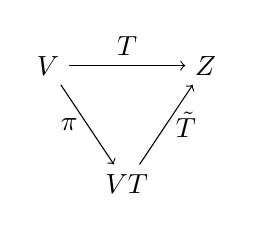
\begin{tikzpicture}
		\node (V) at (-1,1.5) {$V$};
		\node (Z) at (1,1.5) {$Z$};
		\node (K) at (0,0) {$V\quot\Ker T$};
		\draw [->] (V) to node[above]{$T$} (Z);
		\draw [->] (V) to node[left]{$\pi$} (K);
		\draw [->] (K) to node[right]{$\tilde{T}$} (Z);
	\end{tikzpicture}
\end{figure}
\begin{proof}
	L'applicazione $\tilde{T}$ è naturalmente definita come $\tilde{T}(\Ker T+x)=T(x)$.

	Verifichiamo innanzitutto che l'applicazione $\tilde{T}$ sia \emph{ben definita}, ossia che $\tilde{T}(X)$ non dipenda dal rappresentante scelto per la classe	$X$.
	Sia $\Ker T+x\in V\quot\Ker T$, e prendiamo un altro rappresentante $y\in V$, tale che $\Ker T+x=\Ker T+y$: le immagini delle due classi dovranno coincidere.
	Dato che $x\sim y$, risulta $x-y\in\Ker T$, ma allora $\tilde{T}(\Ker T+x)-\tilde{T}(\Ker T+y)=T(x)-T(y)=T(x-y)=0_Z$ cioè $\tilde{T}(\Ker T+x)=\tilde{T}(\Ker T+y)$.
	Analogamente, se per un $w\in V$ si avesse $\Ker T+x\ne\Ker T+w$, allora anche $\tilde{T}(\Ker T+x)\ne\tilde{T}(\Ker T+w)$: è sufficiente notare che se, per assurdo, le immagini coincidessero, allora dovrebbero coincidere anche le preimmagini, poich\'e risulterebbe $x-w\in\Ker T$.
	Quindi l'applicazione è ben definita.

	L'unicità è immediata: supponiamo che esista un'altra applicazione $U\colon V\quot\Ker T\to Z$ tale che $U\big(\pi(x)\big)=T(x)$.
	Per ogni $y\in V\quot\Ker T$ esiste $x\in V$ tale per cui $\pi(x)=y$, dunque $U(y)=U\big(\pi(x)\big)=T(x)=\tilde{T}\big(\pi(x)\big)=\tilde{T}(y)$, ma allora $U=\tilde{T}$.

	Mostriamo ora che è lineare, rispetto alle operazioni nello spazio quoziente introdotte nella sezione \ref{sec:spazi_quoziente}.
	Prendiamo $\Ker T+a,\Ker T+b\in V\quot\Ker T$ e $\lambda\in K$: risulta
	\begin{multline}
		\tilde{T}\big((\Ker T+a)+\lambda(\Ker T+b)\big)=\tilde{T}\big(\!\Ker T+(a+\lambda b)\big)=T(a+\lambda b)=\\=T(a)+\lambda T(b)=\tilde{T}(\Ker T+a)+\lambda\tilde{T}(\Ker T+b)
	\end{multline}
	perciò $\tilde{T}$ è lineare.

	Il nucleo di $\tilde{T}$ è $\Ker\tilde{T}=\{\Ker T+v\in V/\Ker T\colon T(v)=0_Z\}$.
	Ma se $T(v)=0_Z$ allora $v\in\Ker T$, perciò $\Ker T+v=\Ker T+0_V$ ossia $\Ker\tilde{T}=\{\Ker T+0_V\}$: ciò prova che $\tilde{T}$ è iniettiva.

	Se infine prendiamo l'applicazione $T$ solo tra $V$ e la sua immagine $T(V)$, è ovviamente suriettiva.
	Possiamo quindi trovare un'unica applicazione $L\colon V\quot\Ker T\to T(V)$ sfruttando quanto dimostrato finora.
	Se $z\in T(V)$ allora esiste $v\in V$ tale che $T(v)=z$, dunque è sufficiente prendere $a=\Ker T+v$ per ottenere $L(a)=z$, perciò per ogni $z\in T(V)$ troviamo sempre una controimmagine in $L$: ciò prova che $L\colon V\quot\Ker T\to T(V)$ è anche suriettiva, oltre che iniettiva.
	
	Di conseguenza $L\colon V\quot\Ker T\to T(V)$ è un isomorfismo.
\end{proof}

\begin{corollario} \label{cor:nullita-rango}
	Se $V$ ha dimensione finita e $T\in\lin(V,Z)$, allora $\dim V=\dim\Ker T+\dim\Imm T$.
\end{corollario}
\begin{proof}
	Segue facilmente dal teorema precedente e dal \ref{t:dimensione-quoziente}.
\end{proof}
Da quest'ultima formula possiamo dedurre delle proprietà generali su nucleo e immagine di applicazioni vettoriali.
Se $T\in\lin(V,Z)$, distinguiamo alcuni casi.
\begin{itemize}
	\item Se $\dim V>\dim Z$, allora $T$ non può essere iniettiva, infatti $\Imm T\le Z$ implica $\dim\Imm T\le\dim Z$ da cui $\dim\Ker T=\dim V-\dim\Imm T>0$.
	\item Se $\dim V<\dim Z$, allora $T$ non può essere suriettiva, dato che $\dim\Imm T=\dim V-\dim\Ker T\le\dim V<\dim Z$ quindi non può risultare $\Imm T=Z$.
	\item Se $\dim V=\dim Z$, come è per gli endomorfismi (in cui $Z=V$), iniettività e suriettività si implicano a vicenda: se $T$ è iniettiva allora $\dim\Ker T=0$ da cui $\dim\Imm T=\dim Z$, cioè $\Imm T=Z$ quindi $T$ è suriettiva.
		Viceversa, se $T$ è suriettiva allora $\dim\Imm T=\dim Z=\dim V$ da cui $\dim\Ker T=0$ ossia $\Ker T=\{0\}$.
\end{itemize}

\begin{teorema}[Secondo teorema dell'isomorfismo]
	Siano $W,Z$ sottospazi vettoriali di $V$.
	Allora l'applicazione $T\colon (W+Z)\quot Z\to W\quot(W\cap Z)$ definita come
	\begin{equation}
		T(Z+w+z)=W\cap Z+w
	\end{equation}
	è un isomorfismo.
\end{teorema}
\begin{proof}
	Innanzitutto l'applicazione $T$ deve essere ben definita, cioè non deve dipendere dai rappresentanti della classe.
	Prendiamo due elementi $Z+w+z$ e $Z+w'+z'$ (per $z,z'\in Z$ e $w,w'\in W$) i cui rappresentanti sono in relazione tra loro, ossia tali che $w+z-w'-z'\in Z$.
	Chiaramente $z-z'\in Z$, da cui segue che $w-w'\in Z$: ma allora $w-w'\in W\cap Z$ quindi le immagini $W\cap Z+w$ e $W\cap Z+w'$ coincidono (la loro differenza è $W\cap Z+w-W\cap Z+w'=W\cap Z+(w-w')=W\cap Z$ che è l'elemento neutro dello spazio di arrivo).
	Questo prova che $T$ è ben definita.
	
	Verifichiamo che è lineare: presi $z_1,z_2\in Z$, $w_1,w_2\in W$ e $\lambda\in K$ abbiamo\footnote{Nel tornare da $W\cap Z+w$ a $Z+w+z$, la scelta dell'elemento $z$ è arbitraria, poich\'e come elementi dello spazio quoziente $Z+z=Z$ per ogni $z\in Z$, quindi possiamo scegliere proprio $z_1$ e $z_2$ per riottenere le controimmagini.}
	\begin{equation}
		\begin{split}
			T\big(Z+w_1+z_1+\lambda(Z+w_2+z_2)\big)&=T(Z+z_1+\lambda z_2+w_1+\lambda w_2)=\\
			&=W\cap Z+w_1+\lambda w_2=\\
			&=W\cap Z+w_1+\lambda(W\cap Z+w_2)=\\
			&=T(Z+w_1+z_1)+\lambda T(Z+w_2+z_2)
		\end{split}
	\end{equation}
	quindi $T$ è lineare.

	Evidentemente $T$ è suriettiva.
	Il suo nucleo è formato da quegli elementi $Z+w+z$ tali che $W\cap Z+w=0$, ossia $w\in W\cap Z$.
	Allora vale anche $w\in Z$, da cui $w+z\in Z$.
	Di conseguenza $Z+w+z=Z$, cioè è lo zero dello spazio quoziente $(W+Z)\quot Z$.
	Ciò prova che $T$ è anche iniettiva, quindi è un isomorfismo.
\end{proof}
\begin{corollario}[Formula di Grassmann]
	Se gli spazi vettoriali $W$ e $Z$ hanno dimensione finita, allora $\dim(W+Z)=\dim W+\dim Z-\dim(W\cap Z)$.
\end{corollario}
\begin{proof}
	I due spazi $(W+Z)\quot Z$ e $W\quot(W\cap Z)$ dal teorema precedente sono isomorfi, perciò hanno la stessa dimensione.
	Allora per il teorema \ref{t:dimensione-quoziente} si ha che $\dim(W+Z)-\dim Z=\dim W-\dim(W\cap Z)$, da cui la tesi.
\end{proof}

\section{Cambiamento di base}
\label{sec:cambiamento-base}
Prendiamo due basi $\mathcal B=\{e_1,\dots,e_n\}$ e $\tilde{\mathcal B}=\{\tilde e_1,\dots\tilde e_n\}$ in uno spazio vettoriale $V$ di dimensione $n$, finita.
Vogliamo studiare in questa sezione come cambiano i vettori delle coordinate e le matrici associate passando da una base all'altra.
Gli elementi della base $\tilde{\mathcal B}$, essendo elementi di $V$, si scrivono a loro volta come combinazione lineare nella base $\mathcal B$: per ogni $\tilde e_i$ esistono dei coefficienti $L_{ik}$ tali che
\begin{equation}
	\tilde e_i=\sum_{k=1}^nL_{ik}e_k=
	\begin{pmatrix}
		e_1&\cdots&e_n
	\end{pmatrix}
	\begin{pmatrix}
		L_{i1}\\
		\vdots\\
		L_{in}
	\end{pmatrix}.
\end{equation}
Affiancando tutti gli elementi della base $\tilde{\mathcal B}$ scriviamo allora che
\begin{equation}
	\begin{pmatrix}
		\tilde e_1&\cdots&\tilde e_n
	\end{pmatrix}
	=
	\begin{pmatrix}
		e_1&\cdots&e_n
	\end{pmatrix}
	L
	\label{eq:trasformazione-base}
\end{equation}
dove $L$ è la matrice
\begin{equation}
	\begin{pmatrix}
		L_{11}&\cdots&L_{n1}\\
		\vdots&\ddots&\vdots\\
		L_{1n}&\cdots&L_{nn}
	\end{pmatrix}
\end{equation}
la cui $j$-esima colonna contiene le coordinate nella base $\mathcal B$ del vettore $\tilde e_j$ della nuova base.
Tale matrice è associata, chiaramente, a un isomorfismo, poich\'e tutte le sue colonne sono linearmente indipendenti (sono una base per definizione) dunque essendo un endomorfismo iniettivo è automaticamente anche suriettivo; $L$ è dunque sempre invertibile.

Prendiamo ora un vettore $v\in V$, che scriviamo come combinazione lineare $\sum_{k=1}^nv_ke_k$ nella base $\mathcal B$ o anche, simbolicamente, con
\begin{equation}
	\begin{pmatrix}
		e_1&\cdots&e_n
	\end{pmatrix}
	\begin{pmatrix}
		v_1\\
		\vdots\\
		v_n
	\end{pmatrix}.
	\label{eq:vettore-coordinate-base-originale}
\end{equation}
Nell'altra base $\tilde{\mathcal B}$, esisteranno dei coefficienti $\tilde v_k$ tali che
\begin{equation}
	v=\sum_{k=1}^n\tilde v_k\tilde e_k=
	\begin{pmatrix}
		\tilde e_1&\cdots&\tilde e_n
	\end{pmatrix}
	\begin{pmatrix}
		\tilde v_1\\
		\vdots\\
		\tilde v_n
	\end{pmatrix},
\end{equation}
perciò usando la \eqref{eq:trasformazione-base} abbiamo
\begin{equation}
	v=
	\begin{pmatrix}
		\tilde e_1&\cdots&\tilde e_n
	\end{pmatrix}
	\begin{pmatrix}
		\tilde v_1\\
		\vdots\\
		\tilde v_n
	\end{pmatrix}=
	\begin{pmatrix}
		e_1&\cdots&e_n
	\end{pmatrix}
	L
	\begin{pmatrix}
		\tilde v_1\\
		\vdots\\
		\tilde v_n
	\end{pmatrix}
\end{equation}
da cui ricaviamo, uguagliandola alla \eqref{eq:vettore-coordinate-base-originale},
\begin{equation}
	\begin{pmatrix}
		v_1\\
		\vdots\\
		v_n
	\end{pmatrix}
	=L
	\begin{pmatrix}
		\tilde v_1\\
		\vdots\\
		\tilde v_n
	\end{pmatrix}
	\qqq
	\begin{pmatrix}
		\tilde v_1\\
		\vdots\\
		\tilde v_n
	\end{pmatrix}
	=L^{-1}
	\begin{pmatrix}
		v_1\\
		\vdots\\
		v_n
	\end{pmatrix}
	\label{eq:cambiamento-base-vettori-coordinate}
\end{equation}
dunque se $L$ è la matrice che porta la base $\mathcal B$ nella base $\tilde{\mathcal B}$ (secondo la \eqref{eq:trasformazione-base}) allora i vettori delle coordinate si trasformano con l'inversa della matrice, ossia $[v]_{\tilde{\mathcal B}}=L^{-1}[v]_{\mathcal B}$.
Si dice in questo caso che i vettori sono \emph{contravarianti}, poich\'e cambiano in modo ``contrario'' a come cambia la base.

Sia ora $T\colon V\to Z$ un'applicazione lineare, con $V$ di dimensione $n$ e $Z$ di dimensione $m$, definiti sul medesimo campo $K$.
Siano $\mathcal B,\tilde{\mathcal B}$ due basi di $V$ e $\mathcal C,\tilde{\mathcal C}$ due basi di $Z$.
Sia $A\in\mat(m,n,K)$ la matrice associata a $T$ nelle due basi $\mathcal B$ e $\mathcal C$, ossia tale che per $v\in V$
\begin{equation}
	[T(v)]_{\mathcal C}=A[v]_{\mathcal B}.
	\label{eq:matrice-associata-base-originale}
\end{equation}
Se $\tilde A$ è associata a $T$ nelle altre due basi, si ha equivalentemente
\begin{equation}
	[T(v)]_{\tilde{\mathcal C}}=\tilde A[v]_{\tilde{\mathcal B}}.
	\label{eq:matrice-associata-base-trasformata}
\end{equation}
Se ora $L$ è la matrice che porta la base $\mathcal B$ nella $\tilde{\mathcal B}$ e $M$ la matrice che porta $\mathcal C$ in $\tilde{\mathcal C}$ (come nella \eqref{eq:trasformazione-base}) allora sappiamo dalla \eqref{eq:cambiamento-base-vettori-coordinate} che
\begin{equation}
	L[v]_{\tilde{\mathcal B}}=[v]_{\mathcal B}
	\hspace{1cm}\text{e}\hspace{1cm}
	M[T(v)]_{\tilde{\mathcal C}}=[T(v)]_{\mathcal C}
\end{equation}
dunque inserendole nella \eqref{eq:matrice-associata-base-originale} troviamo
\begin{equation}
	M[T(v)]_{\tilde{\mathcal C}}=AL[v]_{\tilde{\mathcal B}}
	\qqq
	[T(v)]_{\tilde{\mathcal C}}=M^{-1}AL[v]_{\tilde{\mathcal B}}
\end{equation}
e per confronto con la \eqref{eq:matrice-associata-base-trasformata} nelle nuove basi otteniamo
\begin{equation}
	\tilde A=M^{-1}AL
	\label{eq:trasformazione-matrice-associata}
\end{equation}
che dà la matrice associata a $T$ nelle basi $\tilde{\mathcal B}$ in partenza e $\tilde{\mathcal C}$ in arrivo a partire dalla matrice associata nelle basi originarie $\mathcal B$ e $\mathcal C$.
In particolare, se $T\in\End(V)$, e scegliamo la stessa base sia in partenza che in arrivo, abbiamo che $\tilde A=L^{-1}AL$ è la matrice associata a $T$ nella nuova base.
Le matrici associate a un endomorfismo in basi differenti sono quindi tutte matrici simili.

Come esempio, prendiamo in $\R^2$ la base canonica $\mathcal B$ e la base
\begin{equation}
	\tilde{\mathcal B}=\left\{
		\begin{bmatrix}
			0\\
			-2
		\end{bmatrix},
		\begin{bmatrix}
			1\\
			2
		\end{bmatrix}
	\right\}
\end{equation}
e l'applicazione lineare $T\colon\R^2\to\R^2$ a cui è associata nella base canonica la matrice
\begin{equation}
	A=
	\begin{pmatrix}
		5&0\\
		1&4
	\end{pmatrix}.
\end{equation}
Per costruire la matrice del cambiamento di base, $L$, dobbiamo prendere le coordinate dei vettori di $\tilde{\mathcal B}$ rispetto alla base $\mathcal B$: poich\'e quest'ultima è la base canonica le coordinate coincidono con le componenti dei vettori stessi, perciò
\begin{equation}
	L=
	\begin{pmatrix}
		0&1\\
		-2&2
	\end{pmatrix}
\end{equation}
di conseguenza la matrice associata a $T$ nella base $\tilde{\mathcal B}$ (in arrivo e in partenza) è
\begin{equation}
	\tilde A=L^{-1}AL=
	\begin{pmatrix}
		1&-\frac12\\
		1&0
	\end{pmatrix}
	\begin{pmatrix}
		5&0\\
		1&4
	\end{pmatrix}
	\begin{pmatrix}
		0&1\\
		-2&2
	\end{pmatrix}
	=
	\begin{pmatrix}
		4&\frac12\\
		0&5
	\end{pmatrix}.
\end{equation}

